%%%%%%%%%%%%%%%%%%%%%%%%%%%%%%%%%%%%%%%%%%%%%%%%%
% Introduction
%%%%%%%%%%%%%%%%%%%%%%%%%%%%%%%%%%%%%%%%%%%%%%%%%
\subsection{Introduction}
\label{hls:introduction}
\nocite{Xilinx:Tutorial}
\gls{HLS} is a process of converting a program that was written in a
higher-level language (such as \programmingLanguage{C},
\programmingLanguage{C++} or \programmingLanguage{SystemC}) into an \gls{RTL}
implementation for use with an \gls{FPGA}. In particular, the \gls{HLS} tool
\software{AutoESL} was used for this Thesis. When synthesising an \gls{RTL}
implementation, there are two competing design goals that could be targeted. The
first is to create a design with the smallest area; the second is a design with
the highest throughput. Each design goal may have a bit emphasis depending on
the nature of the application.

The key advantage of \gls{HLS} tools is that development time for a high-level
programming language is much smaller than development time for a \gls{RTL}
\gls{HDL} programming language \cite{Berkeley:2010}. In addition, programming in
an \gls{RTL} \gls{HDL} programming language is much more error prone and
requires a vastly different skill set. The main criteria that must be considered
when choosing to use a \gls{HLS} tool for hardware development is whether use of
the tool deliver substantial improvements in productivity without compromising
the performance and efficiency of the hardware design.

In \software{AutoESL}, the design flow for \gls{HLS} involves the following
stages \cite{Xilinx:Tutorial}:
\begin{enumerate}
    \item \textbf{Elaboration:} Elaborates the source code into an internal
        database containing operators. The operators represent operations in the
        \programmingLanguage{C} code such as additions, multiplications, array
        reads and writes. See \autoref{hls:operators}.
    \item \textbf{Synthesis:} Maps the operators to cores from the
        \software{AutoESL} library. Cores are the specific hardware components
        used to create the design (such as adders, multipliers, pipelined
        multipliers and block \glspl{RAM}). See \autoref{hls:cores}.
    \begin{enumerate}
        \item \textbf{Scheduling:} Scheduling determines in which cycles
            operations can occur.
        \item \textbf{Binding:} Scheduled operations are bound to specific
            hardware implementations.
    \end{enumerate}
    \item \textbf{Simulation:} Verifies the \gls{RTL} through co-simulation with
        the \programmingLanguage{C} test bench.
    \item \textbf{Implementation:} Generates and executes the scripts to perform
        logic synthesis.
\end{enumerate}

The synthesis process handles a single top level function from the higher-level
language source code as the basis for the \gls{RTL} implementation. The
arguments to this top level functions are synthesised into \gls{RTL} ports
through a process known as interface synthesis \cite{Xilinx:CodingStyleGuide}.
See \autoref{hls:ports} for an explanation of the ports that are available for
interface synthesis.

% TODO: Finish
\begin{figure}
    \centering
    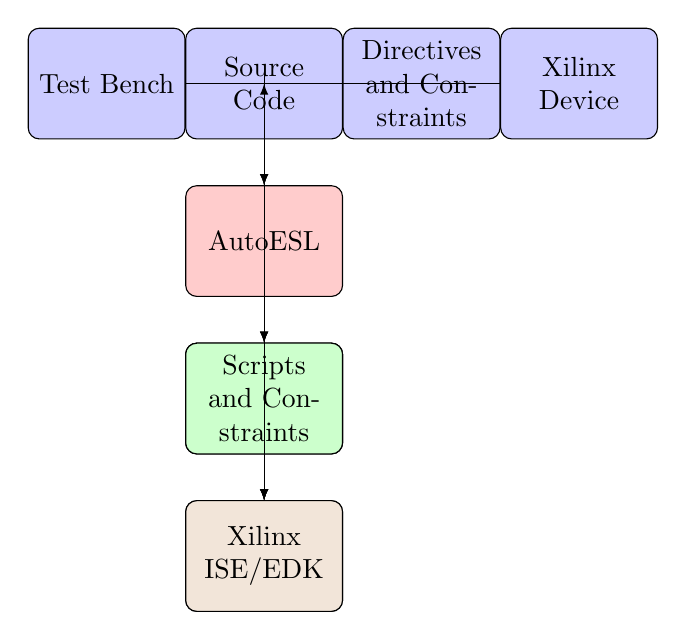
\begin{tikzpicture}[
			block/.style = {
			    rectangle,
			    draw,
                text width = 5em,
                text centered,
                rounded corners,
                minimum height = 4em},
            arrow/.style = {
                draw,
                ->,
                -latex},
            node distance = 2cm]
        % Place nodes
        \node [block, fill=blue!20] (tb) {Test Bench};
        \node [block, fill=blue!20, right of=tb] (insrc) {Source Code};
        \node [block, fill=blue!20, right of=insrc] (dc) {Directives and Constraints};
        \node [block, fill=blue!20, right of=dc] (dev) {Xilinx Device};
        \node [block, fill=red!20, below of=insrc] (aesl) {AutoESL};
        \node [block, fill=green!20, below of=aesl] (rtl) {RTL Wrapper};
        \node [block, fill=green!20, below of=aesl] (outsrc) {Source Code};
        \node [block, fill=green!20, below of=aesl] (sc) {Scripts and Constraints};
        \node [block, fill=brown!20, below of=rtl] (sim) {ModelSim};
        \node [block, fill=brown!20, below of=outsrc] (edk) {Xilinx ISE/EDK};
        
        % Draw edges
        \path [arrow] (tb) -| (insrc);
        \path [arrow] (insrc) -| (aesl);
        \path [arrow] (dc) -| (aesl);
        \path [arrow] (dev) -| (aesl);
        \path [arrow] (aesl) -| (rtl);
        \path [arrow] (aesl) -| (outsrc);
        \path [arrow] (aesl) -| (sc);
        \path [arrow] (tb) -| (sim);
        \path [arrow] (rtl) -| (sim);
        \path [arrow] (outsrc) -| (sim);
        \path [arrow] (outsrc) -| (edk);
        \path [arrow] (sc) -| (edk);
    \end{tikzpicture}
    \caption{AutoESL design flow}
    \label{fig:autoesl:flow}
\end{figure}

\begin{comment}
Interface synthesis automatically handles the data sequencing to and from the design: the user simply needs to select the appropriate interface.
Many types of interfaces can be synthesized: wire ports, single and two-way handshakes, RAM access ports and FIFO ports among others.
\end{comment}

From an \software{AutoESL} synthesised design, Xilinx's \gls{RTL} tools (namely
\gls{ISE} and \gls{EDK}) allow the \gls{RTL} design to be transformed into a
complete \gls{FPGA} design in the form of a bitstream. The Xilinx \gls{HLS}
tools also generate wrappers that allow for the \gls{FPGA} design to be
interfaced with external memory and \gls{IO} resources.

%%%%%%%%%%%%%%%%%%%%%%%%%%%%%%%%%%%%%%%%%%%%%%%%%
% Ports
%%%%%%%%%%%%%%%%%%%%%%%%%%%%%%%%%%%%%%%%%%%%%%%%%
\subsection{Ports}
\label{hls:ports}
\begin{comment}
Clock port
Reset port
Block-level handshaking ports
Output valid signal

A clock and reset port are added to the design.
 AutoESL adds design-level handshake signals by default: ports ap_start, ap_done and ap_idle.
 If the function has a return value, output port ap_return is added to the RTL interface.
 Function arguments which are both read from and written to, are synthesized as separate input and output ports (sum_i and sum_o in Figure 1).
 By default, input pass-by-value arguments and pointers will be synthesized as simple wire ports with no associated handshaking signal.
 By default, output pointers will be synthesized with an associated output valid signal to indicate when the output data is valid.

Basic Pointers
A function with basic pointers on the top-level interface, such as shown in Example 7, produces no issues for HLS. The pointer can be synthesized to either a simple wire interface or an interface protocol using handshakes.

To be synthesized as a FIFO interface, a pointer must be read-only or write-only.

Pointer Arithmetic
The problem with the pointer arithmetic is that it does not access the pointer data in sequence. Wire, handshake or FIFO interfaces have no way of accessing data out of order:
 A wire interface will read data when the design is ready to consume the data or write the data when the data is ready.
 Handshake and FIFO interfaces will read and write when the control signals permit the operation to proceed.

Wire, handshake or FIFO interfaces can only be used on streaming data and therefore cannot be used in conjunction with pointer arithmetic (unless it indexes the data starting at zero and then proceeds sequentially).

Arrays
Alternatively the code must be modified as shown in Example 11, with an array on the interface instead of a pointer. This can be implemented in synthesis with a RAM (ap_memory) interface, which has the capability of indexing the data with an address and can perform out-of-order, or non-sequential accesses.
Arrays on the Interface
In HLS, arrays are synthesized into memory elements by default. When an array is used as an argument to the top-level function the memory is assumed to be “off-chip” and interface ports are synthesized to access the memory.

Modeling Streaming Data Interfaces
Unlike software, the concurrent nature of hardware systems allows them to take advantage of streaming data, where data is continuously supplied to the design and the design continuously outputs data: an RTL design can accept new data before the design has finished processing the existing data.

Interfaces
ap_none - This interface provides no additional handshake or synchronization ports and
can be applied to any function argument type except arrays. This is the default interface
type for all read-only arguments (input ports), except array arguments.
ap_ack - Can be specified on any function argument except arrays and provides an
additional acknowledge port to indicate input data has been read by this RTL block or
confirm output data has been read by a downstream RTL block.
ap_vld - Can be specified on any function argument except arrays and provides an
additional data-valid port to indicate when input data is valid and can be read or when
output data is valid.
ap_ovld - Identical to the ap_vld interface except that it only applies to write-only
arguments (RTL output ports). This is the default interface type for all write-only arguments,
except array arguments.
ap_hs - Implements each argument with an RTL port supported by a full two-way
acknowledge and valid handshake. This can be specified for any function argument except
arrays.
ap_fifo - An ap_fifo interface can be specified for pointer, array or pass-by-reference
arguments. An ap_fifo interface implements the data accesses as reads and writes to a
FIFO, with associated empty, full and data valid signals.
ap_bus - This interface implements pointer and pass-by-reference variables as a general
purpose bus access similar to a typical DMA interface.
ap_memory - This interface is the default type for arrays arguments and can only be
specified on array arguments. An ap_memory interface results in an RTL implementation
which accesses the array elements as data values in a RAM, with associated address, chip
enable and write enable control signals. The set_directive_resource command
should be used to identify which RAM resource in the technology library is used for the
array: this will in turn specify the number of ports available and which control signals are
implemented.
ap_ctrl_none and ap_ctrl_hs - These interface types can only be specified on the
function return argument. The ap_ctrl_hs is the default and adds function level control
signals: an input start signal, output idle and done signals. If there is a function return
argument, the done signal signifies when the return value is valid. The ap_ctrl_none
type ensures these control signals are not added to the design.
\end{comment}

%%%%%%%%%%%%%%%%%%%%%%%%%%%%%%%%%%%%%%%%%%%%%%%%%
% Modules
%%%%%%%%%%%%%%%%%%%%%%%%%%%%%%%%%%%%%%%%%%%%%%%%%
\subsection{Modules}
\label{hls:modules}

%%%%%%%%%%%%%%%%%%%%%%%%%%%%%%%%%%%%%%%%%%%%%%%%%
% Memories
%%%%%%%%%%%%%%%%%%%%%%%%%%%%%%%%%%%%%%%%%%%%%%%%%
\subsection{Memories}
\label{hls:memories}

%%%%%%%%%%%%%%%%%%%%%%%%%%%%%%%%%%%%%%%%%%%%%%%%%
% Expressions
%%%%%%%%%%%%%%%%%%%%%%%%%%%%%%%%%%%%%%%%%%%%%%%%%
\subsection{Expressions}
\label{hls:expressions}

%%%%%%%%%%%%%%%%%%%%%%%%%%%%%%%%%%%%%%%%%%%%%%%%%
% Registers
%%%%%%%%%%%%%%%%%%%%%%%%%%%%%%%%%%%%%%%%%%%%%%%%%
\subsection{Registers}
\label{hls:registers}

%%%%%%%%%%%%%%%%%%%%%%%%%%%%%%%%%%%%%%%%%%%%%%%%%
% Operators
%%%%%%%%%%%%%%%%%%%%%%%%%%%%%%%%%%%%%%%%%%%%%%%%%
\subsection{Operators}
\label{hls:operators}
\nocite{Xilinx:CoreGuide}
% TODO
\begin{description}
\item[add] Addition.
\item[ashr] Arithmetic shift right.
\item[br] Break operation.
\item[fiforead] \gls{FIFO} read.
\item[fifowrite] \gls{FIFO} write.
\item[fifonbread] Non-blocking \gls{FIFO} read.
\item[fifonbwrite] Non-blocking \gls{FIFO} write.
\item[icmp] Integer compare.
\item[load] Memory read.
\item[lshr] Logical shift right.
\item[mul] Multiplication.
\item[mux] Multiplexor.
\item[phi] Multiplexor.
\item[sdiv] Signed divider.
\item[shl] Shift left.
\item[srem] Signed remainder.
\item[store] Memory write.
\item[sub] Subtraction.
\item[udiv] Unsigned division.
\item[urem] Unsigned remainder.
\item[wireread] \gls{IO} read operation.
\item[wirewrite] \gls{IO} write operation.
\end{description}

%%%%%%%%%%%%%%%%%%%%%%%%%%%%%%%%%%%%%%%%%%%%%%%%%
% Cores
%%%%%%%%%%%%%%%%%%%%%%%%%%%%%%%%%%%%%%%%%%%%%%%%%
\subsection{Cores}
\label{hls:cores}
\nocite{Xilinx:CoreGuide}
% TODO
\begin{description}
\item[Functional Unit Cores] Implement standard RTL logic operations (such as
    add, multiply, and compare).
\item[Storage Core] Implement storage elements such as registers or memories.
\item[Connector Cores] Implement connectivity within the design. This includes
    direct connections and streaming storage elements.
\item[Adapter Cores] Implement interfaces used to connect the top-level design
    when \gls{IP} is generated. These interfaces are implemented in the
    \gls{RTL} wrapper used in the \gls{IP} generation flow.
\item[Floating Point Cores] If no floating point core exists for an operator or
    function, \software{AutoESL} will not be able to synthesis the floating
    point operator and synthesis will halt.
\end{description}

%%%%%%%%%%%%%%%%%%%%%%%%%%%%%%%%%%%%%%%%%%%%%%%%%
% Bit Accurate Design
%%%%%%%%%%%%%%%%%%%%%%%%%%%%%%%%%%%%%%%%%%%%%%%%%
\subsection{Bit Accurate Design}
\label{hls:bitAccurate}
Bit accurate types
Arbitrary precision types

%%%%%%%%%%%%%%%%%%%%%%%%%%%%%%%%%%%%%%%%%%%%%%%%%
% Directives
%%%%%%%%%%%%%%%%%%%%%%%%%%%%%%%%%%%%%%%%%%%%%%%%%
\subsection{Directives}
\label{hls:directives}
\nocite{Xilinx:ReferenceGuide}
\software{AutoESL} uses directives (set using either a command in a
\programmingLanguage{tcl} script or using the \command{#pragma} preprocessor
directive) to specify specific \gls{RTL} implementation details or optimizations
that should be applied to the source code. In this section, some of the more
important directives will be described.

\begin{description}
\item[INLINE]
\item[PIPELINE]
\item[TOP]
\item[UNROLL]
\end{description}

